\documentclass{article}

\usepackage[%
    left=0.5in,%
    right=0.5in,%
    top=0.5in,%
    bottom=0.5in,%
]{geometry}%
\usepackage{minitoc}
\usepackage{multicol}
\usepackage{graphicx}
\usepackage{fixltx2e}
\usepackage{listings}
\usepackage{color}
\usepackage{hyperref}
    \hypersetup{ colorlinks = true, linkcolor = blue }
\usepackage{blindtext}
\definecolor{lightgray}{gray}{0.9}
\graphicspath{ {./} }

\newcommand{\inlinecode}[2]{\colorbox{lightgray}{\lstinline
[language=#1]$#2$}}
\newcommand{\worddef}[1]{\hyperref[sec:reference]{\textit{#1}}}

\begin{document}

\tableofcontents

\newpage

\section{IPC}
Inter-process communication. Each process has its own address space. This provides data isolation and prevents direct interaction between different processes. How can we communicate with a Service, or send an Intent? Use \textbf{Binder}.
\begin{itemize}
  \item Underpins most Android communication, i.e. when we use various system capabilities
  \item Kernel driver: provides lightweight RPC (remote procedure calls), data passing. C.f. Linux/Unix signals / pipes / sockets etc. Reading and writing Parcels between processes. Process, user ID authority / trust
  \item Per-process thread pool for handling requests
  \item Synchronous calls between processes
\end{itemize}

\section{Binder}

\subsection{Facilities}

\begin{itemize}
  \item Calls: Simple inter-process messaging system. One-way, two-way
  \item Identifying: PID, UID
  \item Notification: Link to death, Leaked Service connections
  \item Managing: Reference counting, object mapping across processes, sleeping and waking worker threads
  \item Indirect functionality: As a token, sharing fd (file descriptor) to shared memory area
\end{itemize}
\newpage

\subsection{Implementation}

\begin{flushleft}
API for apps
\begin{itemize}
  \item AIDL
  \item Java API wrapper
  \begin{itemize}
    \item  Exposes the IBinder interface
    \item Wraps the middleware layer
    \item Parcelable object marshalling interface
  \end{itemize}
\end{itemize}
Native Middleware
\begin{itemize}
  \item Implements the user space (i.e. within a process) facilities of the Binder framework
  \item Marshalling and unmarshalling of specific data to primitives 
  \item Provides interaction with the Binder kernel driver
\end{itemize}
Kernel driver
\begin{itemize}
  \item Supports ioctl system calls from the middleware
  \item Supports cross-process file operations, memory mapping
  \item Thread pool for each service application for IPC
  \item Mapping of objects between processes via \verb|copy_from_user|, \verb|copy_to_user|
\end{itemize}
\end{flushleft}

\begin{center}
  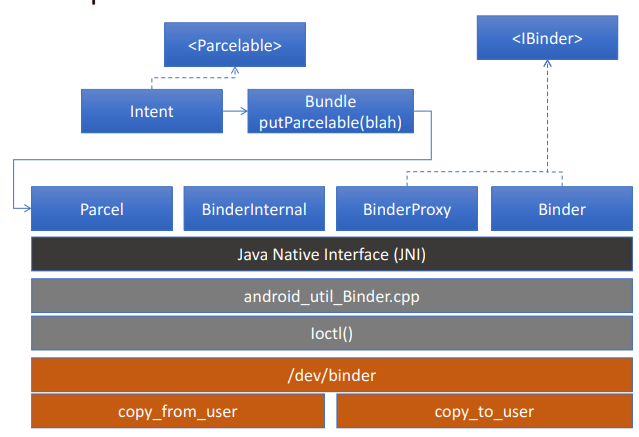
\includegraphics[scale=0.5]{binder_implem.png}
\end{center}

\pagebreak

\subsection{Transactions}
A transaction between processes: IBinder.transact \verb|->| Binder.onTransact(). Binder maintains a pool of transaction threads in each process
\begin{itemize}
  \item To dispatch all IPCs coming from other processes
  \item If process A calls process B
  \begin{itemize}
    \item Calling thread in A blocks in transact()
    \item Sends the transaction to process B
    \item Next available thread in B receives the incoming transaction, calls onTransact() on the target object, replies with the resultant Parcel 
    \item Thread in process A returns, resumes execution
  \end{itemize}
  \item Reliant on Service (B) responding in a timely manner
  \begin{itemize}
    \item Hence catching remote exceptions, transaction failures
    \item Developer defined worker threads
    \item Handling multiple calls from multiple transaction threads
  \end{itemize}
\end{itemize}

\begin{center}
  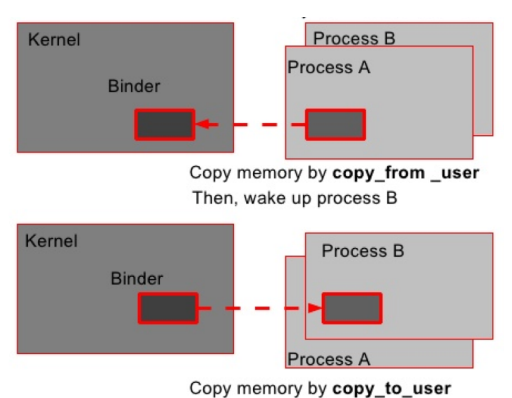
\includegraphics[scale=0.5]{binder_transaction.png}
\end{center}
\begin{center}
  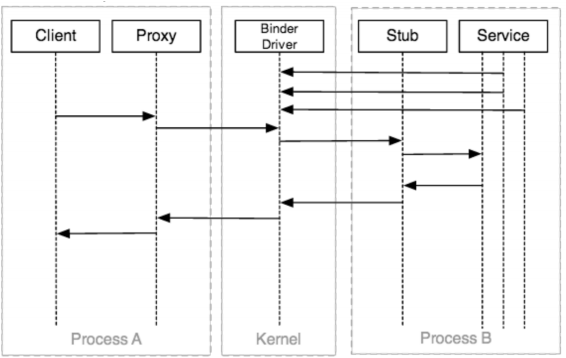
\includegraphics[scale=0.5]{binder_abstraction.png}
\end{center}

\pagebreak

\section{Defining Remotely Bound Services}

\begin{flushleft}
Using the Android Interface Definition Language (AIDL)
\begin{itemize}
  \item Specify an interface for the service functionality
  \item Generates a proxy object
  \item To be used locally as if the remote service was not remote
  \item Generates a stub implementation 
  \item The remote side of the transaction
  \item Generates a communication protocol
  \item Parcelling and unparcelling steps
\end{itemize}
Similar to Java interface definitions. Has label method parameters for efficiency
\begin{itemize}
  \item in: transferred to the remote method
  \item out: returned to the caller
  \item inout: both in and out
  \item oneway: asynchronous
\end{itemize}
Permitted types
\begin{itemize}
  \item Java primitive types, Lists, Maps
  \item Other AIDL-generated interfaces
  \item Classes implementing the Parcelable protocol
\end{itemize}
\end{flushleft}

\section{IPC Abstraction}

\begin{flushleft}
Intent
\begin{itemize}
  \item Highest level abstraction
  \item Asynchronous message passing
\end{itemize}
\textbf{Inter-process} method invocation by using AIDL (Android Interface Definition Language). \textbf{Binder}: kernel driver. \textbf{Ashmem}: Shared memory.
\begin{itemize}
  \item Passed as file descriptor objects by Binder
  \item The USB service gives a specific USB device to an app without giving it unrestricted access
\end{itemize}
\end{flushleft}

\section{Binder Objects and Tokens}
\begin{flushleft}
Binder	Object
\begin{itemize}
  \item An object that can be accessed through the Binder framework
  \item Implements the IBinder interface 
  \item A unique identity maintained across processes
  \begin{itemize}
    \item Allocated by the Binder driver. Cannot be duplicated. Binder objects maintain a unique ID even when parcelled 
    \item A 32 bit handle maintained by the kernel
  \end{itemize}
\end{itemize}
Process A creates a binder object \verb|<-| references memory directly
\begin{itemize}
  \item Passes it to process B \verb|<-| referenced by handle
  \item Passes it to process C \verb|<-| referenced by handle
\end{itemize}
Capability-based security model
\begin{itemize}
  \item Processes are granted access to a particular resource by giving them a capability in the form of the binder object. Binder object as token.
  \item The possession of a token grants the owning process full access to the Binder object enabling it to perform Binder transactions on the target object 
  \item The only way to communicate with a Binder object is to be given a reference to it
\end{itemize}
\end{flushleft}

\section{ServiceManager}

\begin{flushleft}
A	single	context	manager that	maintains	references	to	Binder	objects
\begin{itemize}  
  \item Implemented as ServiceManager
  \item Also hosts many system services within its process 
  \item A Binder instance with a known Binder handle (0) 
  \item Knows about other remote services 
  \begin{itemize}
    \item The first to be registered with Binder 
    \item Only “trusted” system services allowed to register. System, radio, media
  \end{itemize}
\end{itemize}
Client does not know the token of remote Binder. Only the Binder interface \textbf{knows its own address}. Binder submits a service name and its Binder token to the ServiceManager via IPC. Client retrieves remote service Binder handle with service name and communicates with remote service
\end{flushleft}

\begin{center}
  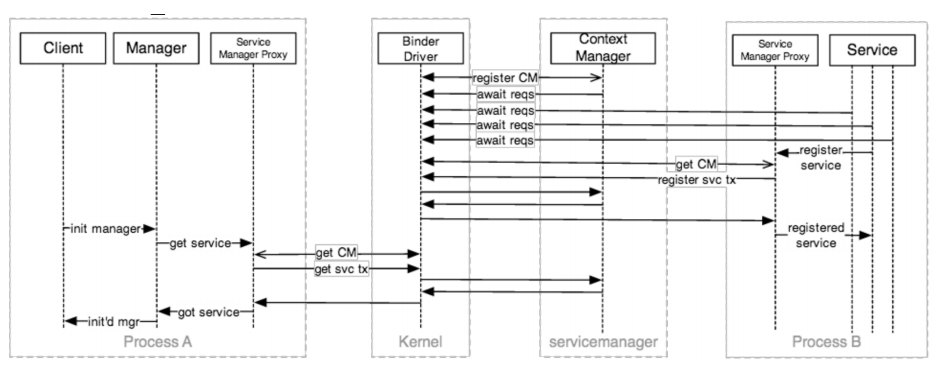
\includegraphics[scale=0.5]{service_manager.png}
\end{center}

\section{Binder}

\subsection{Security}

\begin{flushleft}
Binder	doesn’t	deal	with	security
\begin{itemize}
  \item Enables a trusted execution environment
  \item Transactions via the kernel 
  \item Client identity managed by the kernel 
  \item Binder.getCallingUid(), Binder.getCallingPid() 
  \item UID / PID included in each transcation
\end{itemize}
Access controlled in two ways
\begin{itemize}
  \item Limit who can obtain a reference to a Binder object. Has interface reference security. Client cannot guess “address” of a service without going via the Service Manager.
  \item Check caller identity before performing an action on the Binder object 
  \item Service asks package manager about UID permissions 
  \item Check whether it holds a permission we want to enforce via PackageManager.getPackageInfo(...) 
\end{itemize}
\end{flushleft}
\newpage

\subsection{Performance}

\begin{flushleft}
Explicit limitations
\begin{itemize}
  \item Transactional buffer size 1Mb per process for all concurrent transactions in a process 
  \item Many moderately sized transactions could also exhaust its limit. Arguments and return values are too large 
  \item Keep transaction data small
\end{itemize}
Implicit limitations
\begin{itemize}
  \item Data is copied: duplication of memory resources
  \item Native binary parcelling: better than reflection based serialization, still has overhead of parcel marshalling 
  \item Not ideal for large data-streams, but good enough for window / activity / surface management -> graphics 
  \item Pass file descriptors to shared memory regions (ashmem - Android shared memory)
\end{itemize}
\end{flushleft}

\begin{description}
	\item[placeholder] \hfill \\
\end{description}
\end{document}
